\documentclass{article}

\usepackage[margin=1in,landscape]{geometry}

\usepackage{graphicx}

\usepackage{minted}
\setminted[bash]{
  fontsize=\Large
}
\renewcommand{\theFancyVerbLine}{\large\arabic{FancyVerbLine}}

\usepackage{subfig}

\usepackage{titlesec}
\titleformat*{\section}{\Huge\bfseries\vspace{2ex}}
\titleformat*{\subsection}{\huge\bfseries}

\begin{document}

\section*{Grading: A Journey}
\subsection*{Peter McEvoy \& Sean Konz}

\newpage

\section*{What's the big deal?}
\vspace{2ex}
\begin{minted}{bash}
    $ cd ~/cs107e_home/assignments
    $ vim src/lib/*.c
    $ make clean && make test
\end{minted}

\newpage

\section*{We can fix that}
\vspace{2ex}
\begin{minted}{bash}
    $ for student in $(cat student_usernames.txt) \
      do \
        cd ~/cs107e_home/assignments \
        vim src/lib/*.c \
        make clean && make test \
      done
\end{minted}

\newpage

\section*{Darn, we forgot to git pull}
\vspace{2ex}
\begin{minted}{bash}
    $ for student in $(cat student_usernames.txt) \
      do \
        cd ~/cs107e_home/assignments \
        git pull \
        vim src/lib/*.c \
        make clean && make test \
      done
\end{minted}

\newpage

\section*{What about tracking results?}
\vspace{2ex}
\begin{minted}{bash}
    $ for student in $(cat student_usernames.txt) \
      do \
        cd ~/cs107e_home/assignments \
        git pull \
        vim src/lib/*.c \
        make clean && make test > results.txt \
      done
\end{minted}

\newpage

\section*{???}
\vspace{2ex}
\begin{center}
    \begin{figure}[h]
        \subfloat[]{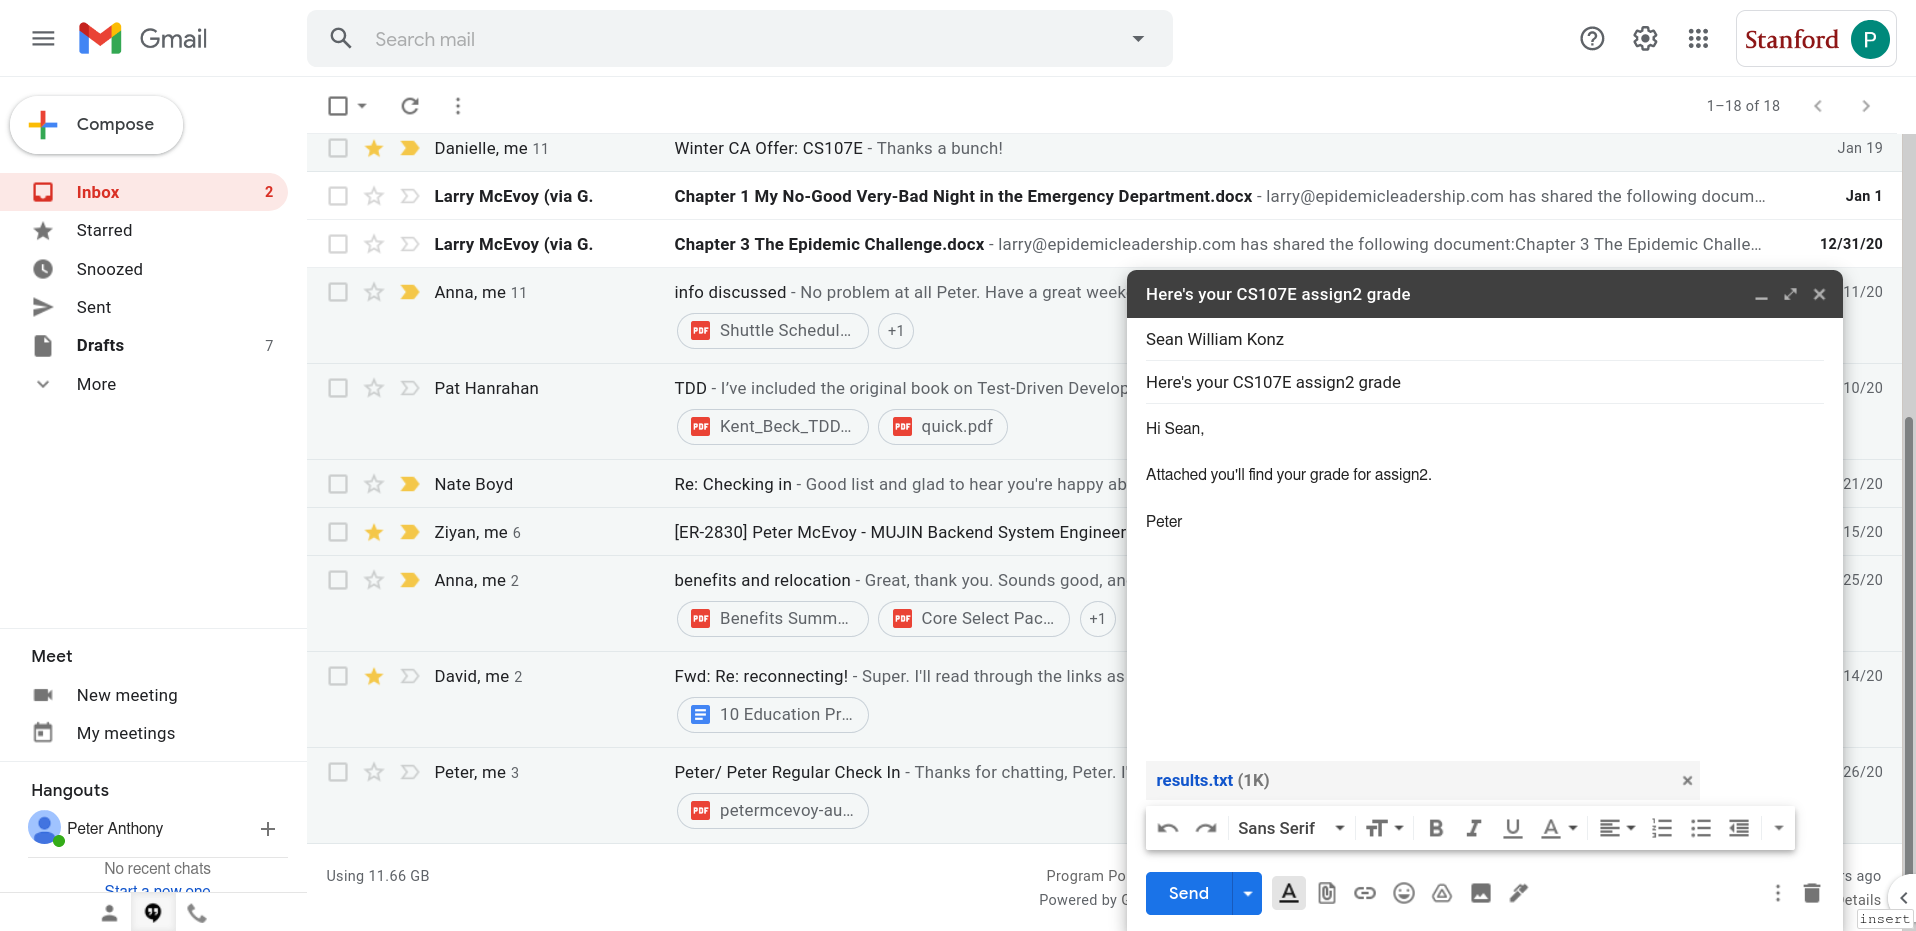
\includegraphics[width=\textwidth]{grades-email.png}}
    \end{figure}
\end{center}

\newpage

\section*{It's more difficult than we thought}
\vspace{2ex}
\begin{minted}{bash}
    // create assignment repos
    // distribute assignment starter code
    // review pull requests
    // test functionality
    // release grades
    // create project repos
    // archive repos
\end{minted}

\newpage

\section*{Someone did this already though, right?}
\vspace{2ex}
\begin{minted}{bash}
    $ ls ~/cs107e_home/logistics/assignments
        archive-project-repos.sh
        archive-repos.sh
        assign0
        assign1
        assign2
        assign3
        assign4
        assign5
        assign6
        assign7
        autograde.py
        averages.py
        collect_scores.py
        compute_late_days.py
        cur_total_scores.csv
        cur_total_scores.json
        delete-assignment-repos.py
        delete-project-repos.py
        deploy.py
        due_dates.py
        generate_csv.py
        generate_grading_assignments.py
        get_late_day_commits.py
        github_names.txt
        grade.py
        grade_stats.py
        initialize_repositories.py
        initialize_travis.py
        init_project_repos.py
        merge_grade.py
        merge_starter_code_commit_to_master.py
        one-offs
        plot_distribution.py
        project
        publish_final_score.py
        README.md
        release_autograde.py
        release.py
        remove_repositories.py
        requirements.txt
        scores_to_csv.py
        style.py
        tag_submission_commits.py
        toolbox
        update_student_repos.py
        utils.py
        who_submitted.py
\end{minted}

\newpage

\section*{If some scripts are good, more scripts must be better}
\vspace{2ex}
\begin{minted}{bash}
    $ ls -l | grep -e '.py' -e '.sh' | wc -l
      31
\end{minted}

\newpage

\section*{C'mon, please?}
\vspace{2ex}
\begin{minted}{bash}
    $ find / -name magical-grading-infrastructure-that-just-works -type d    
\end{minted}

\newpage

\section*{Let's make it less bad}
\vspace{2ex}
\begin{minted}{bash}
$ lsi --help 
    usage: lsi [-h] {add,clone,drop,generate,grade,release,review,test} ...

Run the CS107E grading infrastructure.

optional arguments:
  -h, --help            show this help message and exit

subcommands:
  {add,clone,drop,generate,grade,release,review,test}
                        subcommand help
    add                 add student repos
    clone               clone student repos into $CS107E_STUDENTS_DIR
    drop                drop students from the class or tests from an
                        assignment
    generate            generate grading files
    grade               grade an assignment
    release             release grades for an assignment
    review              copy prewritten pull request comments to the clipboard
                        during code review
    test                build and run assignment tests without grading
\end{minted}

\newpage

\section*{Ta-da}
\vspace{2ex}
\begin{minted}{bash}
$ lsi add students
$ lsi grade quality assign3 -g sean
$ lsi grade functionality assign3 -g sean
$ lsi release assign3 -g sean
$ lsi test list assign4
$ lsi test run assign4 --username swkonz --test-name buggy_malloc_test
$ lsi add project-groups
$ lsi generate grades assign7
\end{minted}

\newpage

\section*{Behind the scenes}
\vspace{2ex}
\begin{minted}{bash}
$ ls ~/cs107e_home/lsi/lsi
add.py
assignments.py
cli.py
clone.py
drop.py
env.py
error.py
generate.py
grade.py
__init__.py
output.py
project.py
release.py
repo.py
review.py
test.py
utils.py
\end{minted}

\newpage

\section*{Behind these other scenes}
\vspace{2ex}
\begin{minted}{bash}
$ ls ~/cs107e_home/assignment-tests
assign0
assign1
assign2
assign3
assign4
assign5
assign6
code-review-comments.json
example-test.c
grading.makefile
Makefile.grading
ps2_emulator
test-framework.h
\end{minted}

\newpage

\section*{Which reminds me}
\vspace{2ex}
\begin{minted}{bash}
$ ls ~/cs107e_home/assignment-tests/assign5
assign5_grading.h
fake_ps2.c                              <========
keyboard_event_mixed_modifier.c
keyboard_event_no_modifier.c
keyboard_event_nonsticky_modifier.c
keyboard_event_sticky_modifier.c
keyboard_next_ascii_modifier.c
keyboard_next_ascii_plain.c
keyboard_next_nonascii.c
keyboard_sequence_press_extended.c
keyboard_sequence_press_nonextended.c
keyboard_sequence_release_extended.c
keyboard_sequence_release_nonextended.c
manifest.ini
ps2_read_all.c
ps2_read_invalid.c
shell_evaluate_echo.c
shell_evaluate_help_peek.c
shell_evaluate_history.c
shell_evaluate_invalid.c
\end{minted}

\newpage

\section*{When in doubt, fake it}
\vspace{2ex}
\begin{minted}{cpp}
// keyboard_event_no_modifier.c
unsigned char scancodes[] = {
    press_and_release(_A),
    press_and_release(_B),
    press_and_release(_C),
    press(_ESC),
    0
};

void run_test(void) {
    read_keyboard_events(sizeof(scancodes));
}

// fake_ps2.c
unsigned char ps2_read(ps2_device_t *dev) {
    // The test defines which scancodes it wants by declaring a null-terminated
    // array within the test file.
    extern unsigned char scancodes[];
    static unsigned int i = 0;

    static bool sent_null = false;

    // Hang after sending the null at the end of the array.
    while (sent_null);
    sent_null = (scancodes[i] == 0);

    return scancodes[i++];
}
\end{minted}

\newpage

\section*{What else can we fake?}
\vspace{2ex}
\begin{minted}{bash}
$ ls ~/cs107e_home/assignment-tests/assign6
assign6_grading.h
console_normal.c
console_scroll.c
console_wrap.c
fake_fb.c                   <========
fb_get.c
fb_swap.c
gl_clear.c
gl_clip.c
gl_color.c
gl_double_buffer.c
gl_draw_char.c
gl_draw_pixel.c
gl_draw_pixel_invalid.c
gl_draw_rect.c
gl_draw_string.c
gl_get.c
gl_padded.c
gl_read_pixel_invalid.c
manifest.ini
\end{minted}

\section*{What else can we fake?}
\vspace{2ex}
\begin{minted}{cpp}
// fake_fb.c
#define MAX_BYTES (512 * 512 * 4)
unsigned char fakebuffer[MAX_BYTES];
unsigned char *red_zone_before, *red_zone_after;
const size_t RZ_SIZE = 128;

static volatile fb_config_t fb __attribute__((aligned(16)));

static unsigned char active_buffer = 0;
static bool double_buffered = false;

void fb_init(unsigned int width, unsigned int height,
             unsigned int depth_in_bytes, fb_mode_t mode) { /* code */ }

void fb_swap_buffer(void) { /* code */ }

void *fb_get_draw_buffer(void) { /* code */ }

void *fb_get_onscreen_buffer(void) { /* code */ }

unsigned int fb_get_depth(void) { return fb.bit_depth / 8; }

unsigned int fb_get_height(void) { return fb.height; }

unsigned int fb_get_width(void) { return fb.width; }

unsigned int fb_get_pitch(void) { return fb.pitch; }

static int memchk(const void *ptr, unsigned char byte, size_t sz) { /* code */ }

bool check_red_zones(void) { /* code */ }
\end{minted}

\newpage

\section*{Can we fake a device with another device?}
\vspace{2ex}
\begin{minted}{bash}
$ ls ~/cs107e_home/assignment-tests/ps2_emulator
Makefile
ps2_emulator.c
ps2_emulator_constants.h
README.md
\end{minted}

\newpage

\section*{Of course we can}
\vspace{2ex}
\begin{minted}{cpp}
// ps2_emulator.c
static void init(unsigned int clk_pin, unsigned int data_pin) { /* code */ }

static void write_bit(unsigned char bit, unsigned int clk_pin,
        unsigned int data_pin) {

    // Write data bit while clock is high.
    gpio_write(data_pin, bit & 1);

    // Delay 5 microseconds before pulling clock low.
#   define US_PER_DATA_TRANSITION 5
    timer_delay_us(US_PER_DATA_TRANSITION);

    // Pull clock low.
    gpio_write(clk_pin, 0);

#   define US_PER_CLK_STATE 50
    timer_delay_us(US_PER_CLK_STATE);

    // Bring clock high.
    gpio_write(clk_pin, 1);

    // Delay before next data transition.
    timer_delay_us(US_PER_CLK_STATE - US_PER_DATA_TRANSITION);
}

static void write_corrupt_scancodes(unsigned int clk_pin,
        unsigned int data_pin) { /* code */ }

static unsigned char wait_for_handshake(unsigned int clk_pin,
        unsigned int data_pin) { /* code */ }

void main(void) { /* code */ }
\end{minted}

\newpage

\section*{What happened in between?}
\vspace{2ex}
\begin{minted}{bash}
commit b90a2a9ab65f3ae04b3e5915f503bc1dfc5c1fba
Author: Peter McEvoy <43772349+mcevoypeter@users.noreply.github.com>
Date:   Mon Feb 10 12:08:57 2020 -0800

    Initial commit

 .gitignore | 129 +++++++++++++++++++++++++++++++++++++++++++++++++++++++++++++++++++++++++++++++++++++++
 README.md  |   2 ++
 2 files changed, 131 insertions(+)
\end{minted}

\newpage

\section*{What happened in between?}
\vspace{2ex}
\begin{minted}{bash}
commit 36773676a49d732105f1b392da692e1a898b5932
Author: Peter McEvoy <pmcevoy@stanford.edu>
Date:   Fri Feb 21 11:23:03 2020 -0800

    Put all assignment metadata in single .json file
    
    `assign_whitelist.json` has been swapped out in favor of
    `assignments.json`. The former only contained files to whitelist,
    whereas the latter contains the app, modules, student test, grading
    tests, and whitelist files. The idea here is that if a future staff
    member wishes to change an aspect of an assignment (i.e. the name of the
    application or which tests get run), then they'll only need to modify
    `assignments.json`.

 assign_whitelist.json | 168 ----------------------------------------------------------------------------
 assignments.json      |  91 +++++++++++++++++++++++++++++++++++++++++
 deploy.py             |  13 +++---
 state.py              |   2 +-
\end{minted}

\newpage

\section*{What happened in between?}
\vspace{2ex}
\begin{minted}{bash}
commit 9b63ac2644bdd0a09be3e55abb81f7d45823ad26
Author: Peter McEvoy <pmcevoy@stanford.edu>
Date:   Fri Feb 21 21:04:41 2020 -0800

    Refactor into object-oriented design
    
    The big change here is the switch from separate files for each step of
    the grading pipeline to having a single file, `workers.py`, define a
    class for each step of the pipeline in addition to a base class that
    contains common variables and methods that are used frequently throughout
    the pipeline. The Deployer class was moved into `workers.py`, but it
    hasn't been updated to leverage its inheritance of the Worker class
    variables and methods.

 lsi.py                  |  38 +++++++---------
 state.py                |  26 -----------
 deploy.py => workers.py | 178 ++++++++++++++++++++++++++++++++++++++++++++++++++++++++++++++++----------
 3 files changed, 172 insertions(+), 70 deletions(-)
\end{minted}

\newpage

\section*{What happened in between?}
\vspace{2ex}
\begin{minted}{bash}
commit b28566e1b3d000c091855b83679152babe61a1bf
Author: Peter McEvoy <pmcevoy@stanford.edu>
Date:   Sat Feb 22 03:17:25 2020 -0800

    Finished app grader
    
    I refactored the Deployer class code so that it now works as a subclass
    of the Worker class. Another big addition on this commit is the execute
    method of the Worker class, which provides a flexible interface for
    running a command as if the user were at the shell. The AppGrader class
    is also mostly finished. I think all that's remaining is to beef up the
    error checking when reading in the grader's deductions.

 assignments.json |  39 +++++++---
 workers.py       | 326 +++++++++++++++++++++++++++++++++++++++++++++++++++------------------------------
 2 files changed, 236 insertions(+), 129 deletions(-)
\end{minted}

\newpage

\section*{What happened in between?}
\vspace{2ex}
\begin{minted}{bash}
commit 002048debc1f39b442cca5a14bb0c564a6a4e5b6
Author: Peter McEvoy <pmcevoy@stanford.edu>
Date:   Mon Mar 16 14:58:03 2020 -0700

    Half-baked version of previous design
    
    Committing all that I came up with prior to the design meeting with Sean
    last week. Given the COVID-19 outbreak, we'll both have lots of time to
    code, and I feel better starting more or less from scratch after having
    the benefit of weeks to think about the best design.

 deploy.py | 23 +++++++++--------------
 lsi.py    |  3 +++
 state.py  |  7 +++++++
 worker.py | 26 ++++++++++++++++++--------
 4 files changed, 37 insertions(+), 22 deletions(-)

\end{minted}

\newpage

\section*{What happened in between?}
\vspace{2ex}
\begin{minted}{bash}
commit 3054ca2311f049e60fc019b7a8f0c1a52c291c72
Author: Peter McEvoy <pmcevoy@stanford.edu>
Date:   Tue Mar 17 16:05:11 2020 -0700

    Half-baked version of new design
    
    Again, I don't like the current design. It's taking too much time to
    find a clean install/setup procedure to make the script easy to use. I'm
    thinking that a Bash script might be easier. Am I crazy?

 .gitignore             |  13 +--
 .grades.json           | 969 -------------------------------------------------------------------------------------------------------------------------------------------------------------------------------------
 .student_usernames.txt |  37 -------
 deploy.py              | 104 --------------------
 grade.py               | 166 -------------------------------
 lsi.py                 | 103 ++++++++++++++------
 requirements.txt       |   1 +
 state.py               |  55 -----------
 worker.py              | 127 ------------------------

\end{minted}

\newpage

\section*{What happened in between?}
\vspace{2ex}
\begin{minted}{bash}
commit e1032a93eaa53a8c9adf88a610bfbab33f550c35
Author: Peter McEvoy <pmcevoy@stanford.edu>
Date:   Thu Mar 19 18:38:37 2020 -0700

    Switched from python to bash
    
    Bash feels like a more natural language for the task at hand. Some of
    the syntax is complicated and dense, but it's well-suited to executing
    lots of shell commands and dealing with json (after I learned jq).

 README.md        |  63 ---------------------------------------------------------------
 lsi.py           | 106 ----------------------------------------------------------------------------------------------------------
 requirements.txt |   1 -
 3 files changed, 170 deletions(-)

\end{minted}

\newpage

\section*{What happened in between?}
\vspace{2ex}
\begin{minted}{bash}
commit 1931479447c41789082ae722677957b463c9b634
Author: Peter McEvoy <pmcevoy@stanford.edu>
Date:   Mon Mar 23 13:29:37 2020 -0600

    Configure bot to commit to student repos
    
    Ensure that the only staff member committing to student repositories is
    CS107E bot.

 README.md               | 2 ++
 scripts/create_repos.sh | 4 ++++
 2 files changed, 6 insertions(+)


\end{minted}

\newpage

\section*{What happened in between?}
\vspace{2ex}
\begin{minted}{bash}
commit 3701b8645f228453e56da1e2b097a4cc7c7139e1
Author: Peter McEvoy <pmcevoy@stanford.edu>
Date:   Wed Mar 25 23:11:23 2020 -0600

    Switch back to python
    
    Command line parser for `create` phase set-up. Adapting the bash scripts
    to python shouldn't be difficult. Hopefully this is the last major
    design shift.

 .gitignore      | 147 +++++++++++++++++++++++++++++++++++++++++++++++++++++++++++++++++++++++++++++++++++++++++++++++++++++++++++++++++++++++++++++++++++++++++++++++----
 lsi.py          |  29 +++++++++++++++++++++++++++++
 lsi/__init__.py |   0
 lsi/create.py   |   4 ++++
 lsi/deploy.py   |   4 ++++
 lsi/grade.py    |   4 ++++
 lsi/release.py  |   4 ++++
 7 files changed, 188 insertions(+), 4 deletions(-)

\end{minted}

\newpage

\section*{What happened in between?}
\vspace{2ex}
\begin{minted}{bash}
commit 474ca7d3ab7f916ffcf0c3cca1b97d25ae7c5b44
Author: Peter McEvoy <pmcevoy@stanford.edu>
Date:   Sun Mar 29 11:05:45 2020 -0600

    Add absolute paths and LSI env var to `state.py`
    
    Change the file paths in `state.py` to be absolute so that `lsi.py` can
    run from any directory. An environment variable pointing to the root of
    the LSI repo was necessary to achieve this.

 lsi/state.py | 10 +++++-----
 1 file changed, 5 insertions(+), 5 deletions(-)

\end{minted}

\newpage

\section*{What happened in between?}
\vspace{2ex}
\begin{minted}{bash}
commit a0360dade102a65703811a72ebf6986eb3f6dd32
Author: Peter McEvoy <pmcevoy@stanford.edu>
Date:   Mon Mar 30 10:56:21 2020 -0600

    Switched from github3.py to curl for GitHub API
    
    To get more information into `.lsi.log`, we switched from the python
    GitHub API wrapper to curl, which generates more information. Logging
    was also updated in the create step.

 grades/assignment_grades.json |  16 ++++++++--------
 lsi.py                        |   5 +++--
 lsi/create.py                 | 101 +++++++++++++++++++++++++++++++++++++++++++++++++++--------------------------------------------------
 lsi/utils.py                  |  19 +++++++++++++------
 4 files changed, 75 insertions(+), 66 deletions(-)

\end{minted}

\newpage

\section*{What happened in between?}
\vspace{2ex}
\begin{minted}{bash}
commit f3c46080796b1a963609589ee22cc9ff9d511377
Author: Peter McEvoy <pmcevoy@stanford.edu>
Date:   Mon Mar 30 13:06:24 2020 -0600

    Beginnings of release phase
    
    Modified `deploy.py` so that the starter code is copied to master, then
    the new branch is created. This allows for a better diff for pull
    requests. The merge functionality in `release.py` seems to be good, but
    I'm not sure. I'm sick of git for the moment.

 grades/assignment_grades.json | 12 ++++++------
 lsi.py                        |  2 ++
 lsi/deploy.py                 | 52 +++++++++++++++++++++++++++++++++-------------------
 lsi/release.py                | 47 ++++++++++++++++++++++++++++++++++++++++++++++-
 4 files changed, 87 insertions(+), 26 deletions(-)

\end{minted}

\newpage

\section*{What happened in between?}
\vspace{2ex}
\begin{minted}{bash}
commit 832171d99f3dcfec2105fc648ae6ed26b8dcd452
Author: Peter McEvoy <pmcevoy@stanford.edu>
Date:   Sat Apr 4 14:09:22 2020 -0600

    Switched back from curl to github3 for GitHub API
    
    Error detection with curl was too weak. Using github3 gives a richer
    ability to report errors, even though there's less information that ends
    up in .lsi.log.

 grades/assignment_grades.json | 129 ++++-----------------------------------------------------------------------------------------------------------------------------
 lsi/create.py                 |  70 ++++++++++++++++++++++++++++++++++++++++++----------------------------
 2 files changed, 46 insertions(+), 153 deletions(-)
\end{minted}

\newpage

\section*{What happened in between?}
\vspace{2ex}
\begin{minted}{bash}
commit fbf879ec9a521a35d1c00ea73cfa849544fd44db
Author: Sean Konz <swkonz@gmail.com>
Date:   Sun Apr 5 22:55:05 2020 -0700

    assignment 2 tests done

    I also added a test template file that should be used as the starter for all test files

 grades/assignments/assign2/test_gpio_get_function.c | 189 ++++++++++++++++++++++++++++++++++++++++++++++++++++++++++++++++++++++++++++++++++++++++++++++++++++++++++++++++++++++++++++++++++++++++++++++++++++
 grades/assignments/assign2/test_gpio_read.c         | 159 ++++++++++++++++++++++++++++++++++++++++++++++++++++++++++++++++++++++++++++++++++++++++++++++++++++++++++++++++++++++++++++
 grades/assignments/assign2/test_gpio_set_function.c | 194 ++++++++++++++++++++++++++++++++++++++++++++++++++++++++++++++++++++++++++++++++++++++++++++++++++++++++++++++++++++++++++++++++++++++++++++++++++++++++
 grades/assignments/assign2/test_gpio_write.c        | 174 ++++++++++++++++++++++++++++++++++++++++++++++++++++++++++++++++++++++++++++++++++++++++++++++++++++++++++++++++++++++++++++++++++++++++
 grades/assignments/assign2/test_timer.c             | 124 +++++++++++++++++++++++++++++++++++++++++++++++++++++++++++++++++++++++++++++++++++++++++++++++++
 grades/assignments/assign2/tests.c                  | 110 --------------------------------------------------------------------------------------
 grades/assignments/test_example_file.c              | 105 ++++++++++++++++++++++++++++++++++++++++++++++++++++++++++++++++++++++++++++++++++
 7 files changed, 945 insertions(+), 110 deletions(-)

\end{minted}

\newpage

\section*{What happened in between?}
\vspace{2ex}
\begin{minted}{bash}
commit b6a22037602e54d0a719fcbde95c6cc2d87a49f9
Author: Sean Konz <swkonz@gmail.com>
Date:   Tue Apr 7 13:20:10 2020 -0700

    working on getting grader makefile to work for all assignments

 grades/assignments/Makefile | 151 +++++++++++++++++++++++++++++++++++++++++++++++++++++++++++++++++++++++++++++++++++++++++++++++++++++++++++++++++++++++++++++++------------------------
 lsi.py                      |   2 ++
 lsi/grade.py                |   1 +
 3 files changed, 130 insertions(+), 24 deletions(-)

\end{minted}

\newpage

\section*{What happened in between?}
\vspace{2ex}
\begin{minted}{bash}
commit 45958a815b2272fb8ce650c82443a74c42321a3a
Author: Sean Konz <swkonz@gmail.com>
Date:   Tue Apr 7 19:50:04 2020 -0700

    making progress on grade script

    Script is ready to integrate with the build process and reading deductions

 grades/assignments/assign2/deductions.json | 88 +++++++++++++++++++++++++++++++++++++---------------------------------------------------
 lsi/grade.py                               | 63 +++++++++++++++++++++++++++++++++++++++++++++++++--------------
 lsi/state.py                               |  1 +
 3 files changed, 87 insertions(+), 65 deletions(-)


\end{minted}

\newpage

\section*{What happened in between?}
\vspace{2ex}
\begin{minted}{bash}
commit fe6320d3ee9f9537e8b74b95d6a3f064567dd5c9
Author: Peter McEvoy <mcevoypeter@outlook.com>
Date:   Thu Apr 9 12:18:13 2020 -0600

    Successfully deployed assign0 starter code
    
    Deploy of assign0 was a success. I forgot to add a student who is
    auditing to `data/course_info.json` before creating the repos and
    deploying, so I had to do theirs manually. I also added a staff-only and
    students-only flag to `lsi.py` so that `lsi/deploy.py` can selectively
    to deploy to students, staff, or both.

 data/course_info.json |  1 +
 lsi.py                |  5 +++++
 lsi/deploy.py         | 13 +++++++++++--
 3 files changed, 17 insertions(+), 2 deletions(-)

\end{minted}

\newpage

\section*{What happened in between?}
\vspace{2ex}
\begin{minted}{bash}
commit 7fc67f1319fed55d8bf2c8a24bdc854ee7bf6418
Author: Sean Konz <swkonz@gmail.com>
Date:   Thu Apr 9 15:39:47 2020 -0700

    trying to get git merge to work consistently

    Sometimes it works, but most of the time it doesn't merge...

 lsi.py       |   8 ++++--
 lsi/grade.py | 295 +++++++++++++++++++++++++++++++++++++++++++++++++++++++++++++++++++++++++++++++++++++++++++++++++++++++++++++++--------------------------------------------------------------------------------
 2 files changed, 177 insertions(+), 126 deletions(-)

\end{minted}

\newpage

\section*{What happened in between?}
\vspace{2ex}
\begin{minted}{bash}
commit c2966659dafe2e163be99d8285919870a0c27fd2
Author: Sean Konz <swkonz@gmail.com>
Date:   Thu Apr 9 16:09:35 2020 -0700

    fix bug in merging... Was just forgetting to actually merge...

 lsi/grade.py | 1 +
 1 file changed, 1 insertion(+)

\end{minted}

\newpage

\section*{What happened in between?}
\vspace{2ex}
\begin{minted}{bash}
commit aee91fd52cfe0afc836006275e831b9a5d937035
Author: Peter McEvoy <mcevoypeter@outlook.com>
Date:   Mon Apr 13 13:52:19 2020 -0600

    Add input function to Log class in `lsi/utils.py`
    
    Add a fifth function to the Log class that identifies a line that
    requires user input. The current implementation has the function read in
    the input and return it so that ANSI escape sequences can be used to
    make the user-inputted text show up in italics. This might not be the
    right decision, however, and is subject to change.

 lsi/utils.py | 69 ++++++++++++++++++++++++++++++++++++++++++++++-----------------------
 1 file changed, 46 insertions(+), 23 deletions(-)

\end{minted}

\newpage

\section*{What happened in between?}
\vspace{2ex}
\begin{minted}{bash}
commit b18a471b4ba4d4b5166d9aa038a7c35200b78a73
Author: Peter McEvoy <mcevoypeter@outlook.com>
Date:   Wed Apr 15 10:40:31 2020 -0600

    Deploy starter code to master first
    
    We had switched from deploying starter code to master and then creating
    the assignment branch to creating the assignment branch and then
    deploying the starter code first. We've switched back to the former to
    make merging easier (fast-forward merge) and also to diff against the
    starter code when reviewing pull request.

 lsi/deploy.py | 3 ++-
 1 file changed, 2 insertions(+), 1 deletion(-)

\end{minted}

\newpage

\section*{What happened in between?}
\vspace{2ex}
\begin{minted}{bash}
commit d3d0ff94e29c1cf648df8e822bef34ec773c7756
Author: Peter McEvoy <mcevoypeter@outlook.com>
Date:   Wed Apr 15 23:53:56 2020 -0600

    Drop use of `tee` in `utils.execute`
    
    We'd been using `tee` to direct stdout and stderr of commands run in
    `utils.execute` to both the stdout and stderr variables in `utils.execute`
    and to `.lsi.log`. This was interfering with the return status of
    commands (i.e. a failed `make` still returned zero), so we dropped the
    use of `tee` in favor of writing the stdout and stderr streams to their
    own log files using python.

 lsi.py       | 12 ++++++++----
 lsi/state.py |  3 ++-
 lsi/utils.py | 12 ++++++++----
 3 files changed, 18 insertions(+), 9 deletions(-)

\end{minted}

\newpage

\section*{What happened in between?}
\vspace{2ex}
\begin{minted}{bash}
commit a8c4f585c536ee8f3f5009b35f4cb3d6379cc246
Author: Peter McEvoy <mcevoypeter@outlook.com>
Date:   Sat Apr 18 15:20:52 2020 -0600

    Add `get_repo_names` to `lsi/utils`
    
    Retrieving the list of repo names from the command line or from
    `data/course_info.json` is needed in `lsi/deploy` and `lsi/release`.
    Refactored to move the shared code into `lsi/utils` under the name
    `get_repo_names`.

 lsi.py         |  9 ++++++++-
 lsi/deploy.py  | 15 ++-------------
 lsi/release.py | 43 +++++--------------------------------------
 lsi/utils.py   | 19 ++++++++++++++++++-
 4 files changed, 33 insertions(+), 53 deletions(-)
\end{minted}

\newpage

\section*{What happened in between?}
\vspace{2ex}
\begin{minted}{bash}
commit 345ed5c5adae75053773ddc0a116565a49e7303f
Author: Peter McEvoy <mcevoypeter@outlook.com>
Date:   Sat Apr 18 16:02:48 2020 -0600

    Convert all json file accesses to use `utils.touch_json`
    
    Searched through the modules in `lsi/` and replaced all `with open(<some
    json> ...)` with a call to `utils.touch_json`.

 lsi/create.py | 13 +++++--------
 lsi/grade.py  |  4 ----
 lsi/utils.py  | 41 +++++++++++++++++++++--------------------
 3 files changed, 26 insertions(+), 32 deletions(-)

\end{minted}

\newpage

\section*{What happened in between?}
\vspace{2ex}
\begin{minted}{bash}
commit ea01c872436f80e9c52c97c317e6df9a5bb777bc
Author: Peter McEvoy <mcevoypeter@outlook.com>
Date:   Sat Apr 18 19:06:15 2020 -0600

    Refactor to add test suite
    
    The parsing functionality in `lsi.py` has been moved into `lsi/parse.py`
    to enable thorough testing. The `tests` subdirectory was also added
    along with `tests/test_parse.py`, which tests the parsing functionality.
    A test file for each of the remaining modules is in the works.

 lsi.py              |  75 +++-------------------
 lsi/parse.py        |  88 +++++++++++++++++++++++++
 tests/test_parse.py | 648 ++++++++++++++++++++++++++++++++++++++++++++++++++++++++++++++++++++++++++++++++++++++++++++++++++++++++++++++++++++++++++++++++++++++++++++++++++++++++++++++++++++++++++++++++++++++++
 3 files changed, 746 insertions(+), 65 deletions(-)

\end{minted}

\newpage

\section*{What happened in between?}
\vspace{2ex}
\begin{minted}{bash}
commit d36eae7a1c0d439b64d9b66bef5fbbd4845efe92
Author: Peter McEvoy <mcevoypeter@outlook.com>
Date:   Thu Apr 23 16:20:09 2020 -0600

    Fix bug in deploy
    
    We used `cp -r -n <starter_code_dir>/* .` to copy the starter code into
    the student repos, but `-n` doesn't overwrite any existing files, so we
    were stuck with the assign1 Makefile after releasing assign2.
    `scripts/patch_deploy.sh` is the bash script that we wrote to make the
    fix. This should eventually be refactored into `lsi/patch.py`, which
    will add a `patch` subcommand to lsi that will allow us to make small
    tweaks like this.

 lsi/deploy.py           | 25 +++++++++++++------------
 scripts/patch_deploy.sh | 21 +++++++++++++++++++++
 2 files changed, 34 insertions(+), 12 deletions(-)

\end{minted}

\newpage

\section*{What happened in between?}
\vspace{2ex}
\begin{minted}{bash}
commit 0277a846544789751a8e46690028eed867399fa9
Author: Peter McEvoy <mcevoypeter@outlook.com>
Date:   Sat Apr 25 09:31:40 2020 -0600

    Fix grader issue in grades database
    
    For a given assignment, only one grader was assigned to grade all
    students. Turned out this is because of a python reference issue: the
    dictionary we were using as a template for a student's grades was being
    changed to latest student even after being assigned to the grades
    database dictionary. The fix was to make a deep copy of the template for
    each student. To facilitate this fix, we added a `--database` flag for
    `create.py` so that it can be run to only create the database.

 grades/assignment_grades.json | 564 ++++++++++++++++++++++++++----------------------------------------------------------------------------------------------------------------------------------------------------
 lsi/create.py                 |  16 ++++-
 lsi/parse.py                  |   2 +
 tests/test_parse.py           |  20 +++++++
 4 files changed, 117 insertions(+), 485 deletions(-)
\end{minted}

\newpage

\section*{What happened in between?}
\vspace{2ex}
\begin{minted}{bash}
commit e2ef98c8c513ebf9cf79fa793d2453d4a6992ec2
Author: Sean Konz <swkonz@gmail.com>
Date:   Sat May 2 16:30:34 2020 -0700

    fix autograder functionality bugs

 lsi/functionality.py | 13 ++++++++++---
 1 file changed, 10 insertions(+), 3 deletions(-)
\end{minted}

\newpage

\section*{What happened in between?}
\vspace{2ex}
\begin{minted}{bash}
commit 563815313f744a5e05d135d7139d5511bf436f9b
Author: Sean Konz <swkonz@gmail.com>
Date:   Sat May 2 16:45:17 2020 -0700

    edit script to add tags on extension branches. This is janky

 scripts/create_tags.py | 20 ++++++++++++++++----
 1 file changed, 16 insertions(+), 4 deletions(-)


\end{minted}

\newpage

\section*{What happened in between?}
\vspace{2ex}
\begin{minted}{bash}
commit c51f70da57fd9005af680203985a9e12b24e7a48
Author: Peter McEvoy <mcevoypeter@outlook.com>
Date:   Sat May 9 15:35:49 2020 -0600

    Remove array literal in `test_strings.c`
    
    gcc uses a memcpy when creating a literal array. When we're testing the
    student's memcpy, this is bad news. To get around this, individually
    assign each function pointer into the function pointer array so that gcc
    uses a `ldr` and `str` rather than `memcpy`.

 grades/assignments/assign3/test_strings.c | 40 ++++++++++++++++++++++++++++++++++++----
 1 file changed, 36 insertions(+), 4 deletions(-)

\end{minted}

\newpage

\section*{What happened in between?}
\vspace{2ex}
\begin{minted}{bash}
commit e4f0bf14732291c49a6cd939467385017111c9b3
Author: Sean Konz <swkonz@gmail.com>
Date:   Sat May 9 14:55:21 2020 -0700

    upgrades on grade script to prevent student code usage, issues on branch selection

 grades/assignment_grades.json                       | 624 ++++++++++++++++++++++++++++++++++++++++++++++++++++++++++++++++++++++++++++++++++++++++++++++++++++++++++++++++++++++++++++++++++++++++++++++++--------
 grades/assignments/assign2/test_gpio_get_function.c |   2 +-
 grades/assignments/assign2/test_gpio_read.c         |   2 +-
 grades/assignments/assign2/test_gpio_set_function.c |   2 +-
 grades/assignments/assign2/test_gpio_write.c        |   2 +-
 grades/assignments/assign2/test_timer.c             |   2 +-
 grades/assignments/assign3/deductions.json          | 138 +++++++++++++++++-----------------
 grades/assignments/assign3/test_snprintf.c          |  31 ++++----
 grades/assignments/assign3/test_strings.c           |  55 ++++++++++++--
 grades/assignments/assign3/test_to_base.c           |  28 ++-----
 grades/assignments/test_example_file.c              |   6 +-
 lsi/functionality.py                                |  21 +++++-
 lsi/grade.py                                        |   2 +-
 13 files changed, 759 insertions(+), 156 deletions(-)
\end{minted}

\newpage

\section*{What happened in between?}
\vspace{2ex}
\begin{minted}{bash}
commit f4cf38c1f52c835809427bfd3356f15b240536dd
Author: Sean Konz <swkonz@gmail.com>
Date:   Mon May 11 23:03:58 2020 -0700

    refund student grades for bug in snprintf implementation

 grades/assignment_grades.json | 124 +++++++++++++---------------------------------------------------------------------------------------------------------------
 1 file changed, 13 insertions(+), 111 deletions(-)


\end{minted}

\newpage

\section*{What happened in between?}
\vspace{2ex}
\begin{minted}{bash}
commit 1febd469b6ae774516b3caee626275bd6dbaab0b
Author: Peter McEvoy <mcevoypeter@outlook.com>
Date:   Thu May 14 15:31:22 2020 -0600

    First pass at keyboard emulator
    
    This isn't working, but I suspect I might have an issue with my
    hardware. I'm unable to communicate from one pi to another using a GPIO
    pin.

 grades/assignments/keyboard-emulator/Makefile            |  47 +++++++++++++++++++++++++++++++++++++++++++++++
 grades/assignments/keyboard-emulator/cstart.c            |  26 ++++++++++++++++++++++++++
 grades/assignments/keyboard-emulator/key-em.c            | 147 +++++++++++++++++++++++++++++++++++++++++++++++++++++++++++++++++++++++++++++++++++++++++++++++++++++++++++++++++++++++++++++++++++++++++++++++++++
 grades/assignments/keyboard-emulator/key-em.h            |  16 ++++++++++++++++
 grades/assignments/keyboard-emulator/keyboard-emulator.c |  22 ++++++++++++++++++++++
 grades/assignments/keyboard-emulator/memmap              |  10 ++++++++++
 grades/assignments/keyboard-emulator/start.s             |   6 ++++++
 7 files changed, 274 insertions(+)


\end{minted}

\newpage

\section*{What happened in between?}
\vspace{2ex}
\begin{minted}{bash}
commit 26826f980356cc77ddf7517853d117c60b8584d0
Author: Peter McEvoy <mcevoypeter@outlook.com>
Date:   Sun May 24 17:55:10 2020 -0600

    Simplify keyboard emulator design
    
    In the process of simplifying the keyboard emulator design by creating a
    set of inlined, header files.

 grades/assignments/keyboard-emulator/Makefile            |  11 ++++++-----
 grades/assignments/keyboard-emulator/gpiofast.h          |  77 ++++++++++++++++++++++++++++++++++++++++++++++++++++++++++++++++++++++++++
 grades/assignments/keyboard-emulator/key-em.c            | 154 ---------------------------------------------------------------------------------------------------------------------------------------------------
 grades/assignments/keyboard-emulator/key-em.h            | 130 +++++++++++++++++++++++++++++++++++++++++++++++++++++++++++++++++++++++++++++++++++++++++++++++++++++++++++++++++-----------
 grades/assignments/keyboard-emulator/keyboard-emulator.c |  20 ++++---------------
 grades/assignments/keyboard-emulator/timerfast.h         |  29 ++++++++++++++++++++++++++++
 6 files changed, 235 insertions(+), 186 deletions(-)


\end{minted}

\newpage

\section*{What happened in between?}
\vspace{2ex}
\begin{minted}{bash}
commit ee26c002d930ccb85c976e6f1bf453247ad79de7
Author: Peter McEvoy <mcevoypeter@outlook.com>
Date:   Mon Jun 1 17:49:36 2020 -0600

    Finished grading fb.c and gl.c

 grades/assignment_grades.json              | 137 +++++++++++++++++++++++++++++++++++++++++++++++++++++++++++++++++++++++++++++++++++++++++++++++++++++++++++++++++++++++++++++++----------
 grades/assignments/assign6/deductions.json | 118 +++++++++++++++++++++++++++++++++++++++++++++++++++++++++++++++++++++++++++++++++++++++++++++++++++++++++++++++++++++-
 2 files changed, 244 insertions(+), 11 deletions(-)


\end{minted}

\newpage

\section*{What happened in between?}
\vspace{2ex}
\begin{minted}{bash}
commit cc28744e3b527eb30d4535d14f0ac527864bbd48
Author: Peter McEvoy <mcevoypeter@outlook.com>
Date:   Thu Jun 4 15:42:30 2020 -0600

    Increase timeout on malloc robustness tests
    
    Some of our tests were unconditionally failing because of timeout
    issues.

 grades/assignments/assign4/deductions.json | 8 ++++----
 1 file changed, 4 insertions(+), 4 deletions(-)


\end{minted}

\newpage

\section*{What happened in between?}
\vspace{2ex}
\begin{minted}{bash}
commit fa3a9b7aed42d2bc5e90754c1e125a9e0c8bffa4
Author: Peter McEvoy <mcevoypeter@outlook.com>
Date:   Mon Jun 8 16:13:02 2020 -0600

    Assign5 scripts and traces
    
    Had to grade assign5 by hand, so here is the "infrastructure" that I
    used to do so.

 grades/assignments/assign5/basic.script                 | 23 +++++++++++++++++++++++
 grades/assignments/assign5/extension.script             |  6 ++++++

\end{minted}

\newpage

\section*{What happened in between?}
\vspace{2ex}
\begin{minted}{bash}
commit 14448726ed71ab9a1062aae21d07d2bb59a33d72
Author: Peter McEvoy <mcevoypeter@outlook.com>
Date:   Mon Jun 8 16:14:35 2020 -0600

    [in-progress] keyboard emulator
    
    This is by no means complete, but I'm adding my work on the keyboard
    emulator should we need to build on it for future quarters.

 grades/assignments/keyboard-emulator/key-em.c            |   7 ++-
 grades/assignments/keyboard-emulator/key-em.h            | 376 +++++++++++++++++++++++++++++++++++++++++++++++++++++++++++++++++++++++++++++++++++++++++++++++++++++++++++++++++++++++++++++++++++++++++++++++++--
 grades/assignments/keyboard-emulator/keyboard-emulator.c |   5 +-
 3 files changed, 377 insertions(+), 11 deletions(-)
\end{minted}

\newpage

\section*{What happened in between?}
\vspace{2ex}
\begin{minted}{bash}
commit c2f32086f872f3fcf3a4a570eafcfe2b696cd0be
Author: Peter McEvoy <mcevoypeter@outlook.com>
Date:   Mon Jun 8 16:16:07 2020 -0600

    Assign6 traces
    
    Also had to grade assign6 by hand.

\end{minted}

\newpage

\section*{What happened in between?}
\vspace{2ex}
\begin{minted}{bash}
    commit 1ceebcbbb815956c11cb9408024c2b693c551e2a
Author: Peter McEvoy <mcevoypeter@outlook.com>
Date:   Wed Sep 9 11:43:34 2020 -0600

    Create build system and testing framework
    
    For each test in the given assignment's subdirectory, build two versions
    of the test--one staff, one student--in the given student's repo, run
    each version, collect the output in the given student's repo, diff the
    two outputs, and collect the results ("pass" or "fail") for each test in a results
    file within the given student's repo.
    
    Define the testing framework in `test-framework.h` to minimize the
    amount of boiler plate code needed to write assignment tests. Include an
    example test in `example-test.c`.

 Makefile         | 111 ++++++++++++++++++++++++++++++++++++++++++++++++++++++++++++++++++++++++++++++++++++++++++++++-----------------
 example-test.c   |  15 +++++++++++++++
 test-framework.h |  21 +++++++++++++++++++++
 3 files changed, 130 insertions(+), 17 deletions(-)
\end{minted}

\newpage

\section*{What happened in between?}
\vspace{2ex}
\begin{minted}{bash}
commit 6b3c8ba250701c0bb0a6a71060010efe4a45d2a4
Author: Peter McEvoy <mcevoypeter@outlook.com>
Date:   Sat Sep 12 12:01:30 2020 -0600

    [in-progress] tune up for fall 2020
    
    Remove all of the assignment test files since assignment tests now live
    in a separate repo, `assignment-tests`.
    
    Remove the `scripts` directory, which contained hacky one-off scripts
    that shouldn't be used again.
    
    Remove `deploy.py` and the accompanying deploy-related code in
    `parse.py` and `test_parse.py` since we no longer need an explicit
    deploy action now that we have `assignments-mirror`.
    
    Rewrite the module that creates the grades csv from the grades json so
    that it is more easily understandable.
    
    Add clone subcommand to create local copies of the student repos.
    
    Rewrite the function in the release module that inserts grades into the
    student's README.md so that we can handle a more prettily formatted
    README.md.
    
    Add checkout_branch function to utils module and adopt it in release
    module.
    
    Remove dependency on github3.py from utils and release modules.
\end{minted}

\newpage

\section*{What happened in between?}
\vspace{2ex}
\begin{minted}{bash}
commit 02b476dd51756183150a2027ac93b6e652ecd3d4
Author: Peter McEvoy <mcevoypeter@outlook.com>
Date:   Sat Sep 19 18:28:20 2020 -0600

    Add update-branch and debug targets to Makefile
    
    Update the branch to be graded from within the Makefile. This gets us
    one step closer to completely abstracting away the running of the tests
    from the LSI python driver. Also add a debug target that prints out all
    of the Makefile's macros.

 Makefile | 110 ++++++++++++++++++++++++++++++++++++++++++++++++++++++++++++++++++++++++++++++++++----------------------------
 1 file changed, 82 insertions(+), 28 deletions(-)

\end{minted}

\newpage


\section*{What happened in between?}
\vspace{2ex}
\begin{minted}{bash}
commit 3395a2e45f774f46cb824a98ccecccf20d2b481e
Author: Peter McEvoy <mcevoypeter@outlook.com>
Date:   Mon Sep 28 17:08:40 2020 -0600

    Change due dates to ISO format
    
    The GitHub API returns datetimes in the ISO format. To make things
    easier in the grade module, update the due dates in `course_info.json`
    to also adopt the ISO format. Use `isoformat` in `dateutil.parser`
    module to parse ISO formatted strings into datetime objects.

 course_info.json | 16 ++++++++--------
 lsi/state.py     |  3 ---
 requirements.txt |  1 +
 3 files changed, 9 insertions(+), 11 deletions(-)
\end{minted}

\newpage

\section*{What happened in between?}
\vspace{2ex}
\begin{minted}{bash}
commit e8f75aa892ac0b3c8ea7097e35227cadf6d3bf47
Author: Peter McEvoy <mcevoypeter@outlook.com>
Date:   Fri Oct 2 13:42:34 2020 -0600

    Convert due dates to 24-hour time in course info json
    
    `compute_late_days` in the assignments module failed to correctly
    compute the late days because the assignments were due at 11:59am on
    Tuesday, not 11:59pm.

 course_info.json | 16 ++++++++--------
 1 file changed, 8 insertions(+), 8 deletions(-)


\end{minted}

\newpage

\section*{What happened in between?}
\vspace{2ex}
\begin{minted}{bash}
commit 33dcc7080c28dca77e5f252bb18f651b1c4a54d6
Author: Peter McEvoy <mcevoypeter@outlook.com>
Date:   Fri Oct 2 14:09:37 2020 -0600

    Add output module
    
    Add output module that contains the `log` function, which will be used
    as a function decorator to clean up the code base and remove all of the
    ugly calls to `log.*(...)`.

 lsi/output.py | 60 ++++++++++++++++++++++++++++++++++++++++++++++++++++++++++++
 1 file changed, 60 insertions(+)

\end{minted}

\newpage

\section*{What happened in between?}
\vspace{2ex}
\begin{minted}{bash}
commit 97dd53795c2368cbc4edd1391873c710fd631210
Author: Peter McEvoy <mcevoypeter@outlook.com>
Date:   Sun Oct 11 11:29:10 2020 -0600

    Replace long flags with short flags in Makefile
    
    Some long flags available on Linux are apparently not available on
    macOS.

 Makefile | 23 +++++++++++------------
 1 file changed, 11 insertions(+), 12 deletions(-)


\end{minted}

\newpage


\section*{What happened in between?}
\vspace{2ex}
\begin{minted}{bash}
commit a0ea0b4b50b6c617b47a71c8a7dbc9f5f7fb4183
Author: Peter McEvoy <mcevoypeter@outlook.com>
Date:   Mon Oct 12 00:21:55 2020 -0600

    Fix insidious pipe max output bug in utils.execute
    
    Unix pipes apparently have a max output capacity of 65K, which we exceed
    when invoking the assignment-tests Makefile during the test-running
    portion of the grade module.
    https://thraxil.org/users/anders/posts/2008/03/13/Subprocess-Hanging-PIPE-is-your-enemy/

 lsi/utils.py | 22 ++++++----------------
 1 file changed, 6 insertions(+), 16 deletions(-)

\end{minted}

\newpage

\section*{What happened in between?}
\vspace{2ex}
\begin{minted}{bash}
commit 71a685874fb0d1731867e256be55af4f9a6f0c68
Author: Peter McEvoy <mcevoypeter@outlook.com>
Date:   Sun Oct 18 10:44:14 2020 -0600

    Cache staff results in $CS107E_ASSIGNMENTS_MIRROR_REPO
    
    Run the staff version of the tests once and stick the results in
    $CS107E_ASSIGNMENTS_MIRROR_REPO.

 Makefile | 120 +++++++++++++++++++++++++++++++++++++++++++++++++++++++++++++++++++++++++++++++++++++-----------------------------------
 1 file changed, 85 insertions(+), 35 deletions(-)


\end{minted}

\newpage

\section*{What happened in between?}
\vspace{2ex}
\begin{minted}{bash}
    commit d6e02785c7f0ca849e68814304aab920a923b000
Author: Peter McEvoy <mcevoypeter@outlook.com>
Date:   Sun Oct 25 19:00:41 2020 -0600

    First version of keyboard emulator

 keyboard-emulator/Makefile                |  55 +++++++++++++++++++++++++++++++++++++++++++++++++++++++
 keyboard-emulator/cstart.c                |  26 ++++++++++++++++++++++++++
 keyboard-emulator/fast-gpio.h             |  80 ++++++++++++++++++++++++++++++++++++++++++++++++++++++++++++++++++++++++++++++++
 keyboard-emulator/fast-pi.h               |  45 +++++++++++++++++++++++++++++++++++++++++++++
 keyboard-emulator/fast-timer.h            |  21 +++++++++++++++++++++
 keyboard-emulator/key-em.h                | 126 ++++++++++++++++++++++++++++++++++++++++++++++++++++++++++++++++++++++++++++++++++++++++++++++++++++++++++++++++++++++++++++++
 keyboard-emulator/keyboard-emulator.c     |  31 +++++++++++++++++++++++++++++++
 keyboard-emulator/memmap                  |  10 ++++++++++
 keyboard-emulator/scancode-sequence-500.h |  14 ++++++++++++++
 keyboard-emulator/scancode-sequences.h    |  11 +++++++++++
 keyboard-emulator/scancodes.h             | 132 ++++++++++++++++++++++++++++++++++++++++++++++++++++++++++++++++++++++++++++++++++++++++++++++++++++++++++++++++++++++++++++++++++++
 keyboard-emulator/start.s                 |   6 ++++++
 scancodes-example.h                       |   9 +++++++++
 13 files changed, 566 insertions(+)


\end{minted}

\newpage

\section*{What happened in between?}
\vspace{2ex}
\begin{minted}{bash}
commit 691c50de1beebff59aaca7c1847fe2e2b198edab
Author: Peter McEvoy <mcevoypeter@outlook.com>
Date:   Thu Oct 29 18:34:53 2020 -0600

    Check keyboard emulator clock with logic analyzer

 keyboard-emulator/key-em.h            | 3 +--
 keyboard-emulator/keyboard-emulator.c | 2 +-
 2 files changed, 2 insertions(+), 3 deletions(-)


\end{minted}

\newpage




\section*{What happened in between?}
\vspace{2ex}
\begin{minted}{bash}
commit 0516bcc9f772c3534c79edb98c27665d93cb3b4a
Author: Peter McEvoy <mcevoypeter@outlook.com>
Date:   Mon Nov 2 11:32:20 2020 -0700

    Update assign5 keyboard tests
    
    Keyboard emulator is now up and running. The fix: use the appropriate
    keyboard_init function. If using ref_keyboard_*, then use
    ref_keyboard_init. Same for the non ref_ keyboard implementation.

\end{minted}

\newpage



\section*{What happened in between?}
\vspace{2ex}
\begin{minted}{bash}
Author: Peter McEvoy <mcevoypeter@outlook.com>
Date:   Tue Nov 24 11:26:48 2020 -0700

    Refactor cli.py to use shared parsers

 lsi/cli.py | 137 +++++++++++++++++++++++++++++++++++++++++++++++++++++++++++++----------------------------------------------------------------------------
 1 file changed, 61 insertions(+), 76 deletions(-)

\end{minted}

\newpage

\section*{What happened in between?}
\vspace{2ex}
\begin{minted}{bash}
commit 6185e9b5903cd2fb7a8e85c30ff369debc535fa2
Author: Sean Konz <swkonz@gmail.com>
Date:   Tue Dec 1 11:52:02 2020 -0800

    fix late day script

 compute_late_days.py | 14 +++++++++++++-
 1 file changed, 13 insertions(+), 1 deletion(-)

\end{minted}

\newpage

\section*{What happened in between?}
\vspace{2ex}
\begin{minted}{bash}
commit 9e8508dbde1c3cce3174aa077620837827e2cb7f
Author: Peter McEvoy <mcevoypeter@outlook.com>
Date:   Fri Dec 4 14:19:39 2020 -0700

    Move subparser creation into command modules
    
    Each module that defines a subcommand of lsi now must implement the
    `add_cli_parser` function so that its subparser can be added to the top
    level parser by `cli.py`.

 lsi/add.py      | 68 ++++++++++++++++++++++++++++++++++++++++++++++++++++++++++++++++++++
 lsi/cli.py      | 81 +++++++--------------------------------------------------------------------------
 lsi/clone.py    | 44 ++++++++++++++++++++++++++++++++++++++++++--
 lsi/drop.py     | 23 +++++++++++++++++++++++
 lsi/generate.py | 41 +++++++++++++++++++++++++++++++++++++++++
 lsi/grade.py    | 82 ++++++++++++++++++++++++++++++++++++++++++++++++++++++++++++++++++++++++++++++++++
 lsi/release.py  | 15 +++++++++++++++
 lsi/review.py   | 14 ++++++++++++++
 8 files changed, 292 insertions(+), 76 deletions(-)

\end{minted}

\newpage

\section*{What happened in between?}
\vspace{2ex}
\begin{minted}{bash}
commit 854b1c61a3e4abb9b0cecde3116f08cbbf8e3066
Author: Peter McEvoy <mcevoypeter@outlook.com>
Date:   Wed Dec 23 13:54:27 2020 -0700

    Strip remaining code in assignments.Repo and add TODOs

 lsi/assignments.py | 166 +++++++++++++++++++++++++++++++++++++++++++++-------------------------------------------------------------------------------------------------------------------------
 1 file changed, 45 insertions(+), 121 deletions(-)

\end{minted}

\newpage

\section*{What happened in between?}
\vspace{2ex}
\begin{minted}{bash}
commit d9c12e22fb9a98e199aed2d2ca6ad3b98fa67104
Author: Peter McEvoy <mcevoypeter@outlook.com>
Date:   Mon Jan 18 13:36:49 2021 -0700

    Replace autonomous makefile with makefile stub
    
    Simplify the test build process by replacing the previously humongous
    makefile with a simpler one designed to be included into the student's
    existing makefile.

 Makefile         | 466 -------------------------------------------------------------------------------------------------------------------------------------------------------------------------------------------
 grading.makefile |  59 ++++++++++++++++++++++++
 2 files changed, 59 insertions(+), 466 deletions(-)


\end{minted}

\newpage


\section*{What happened in between?}
\vspace{2ex}
\begin{minted}{bash}
commit ae3d6e40ef2ad53bb6b6586e3afd3651fa52d354
Author: Sean Konz <swkonz@gmail.com>
Date:   Sun Jan 31 08:08:03 2021 -0800

    update assign db format

 assignment_grades.json | 180 ++++++++++++++++++++++++++++++++++++++++++++++++++++++++++++++++++++++++++++++++++++++++++++++++++++++++++++++++++++++++++++++++++++++++++------------------------------------------
 1 file changed, 138 insertions(+), 42 deletions(-)


\end{minted}

\newpage

\section*{What happened in between?}
\vspace{2ex}
\begin{minted}{bash}
commit cb51fccc12f1aec5a9364a16291904fad0be5e11
Author: Sean Konz <swkonz@gmail.com>
Date:   Sun Jan 31 18:20:37 2021 -0800

    Update how we fetch tags to force update refspec

 assignment_grades.json | 188 ++++++++++++++++++++++++++++++++++++++++++++++++++++++++++++++++++++++++++++++++++++++++++-------------------------------------------------------------------------------------------
 lsi/repo.py            |   2 +-
 2 files changed, 95 insertions(+), 95 deletions(-)

\end{minted}

\newpage

\section*{What happened in between?}
\vspace{2ex}
\begin{minted}{bash}
commit 27e6faa51e45f14a5e0361963d6134b8a5665dc7
Author: Sean Konz <swkonz@gmail.com>
Date:   Mon Feb 1 15:46:30 2021 -0800

    fix crashing bug and update grade report language

 lsi/assignments.py | 6 ++++++
 1 file changed, 6 insertions(+)


\end{minted}

\newpage

\section*{What happened in between?}
\vspace{2ex}
\begin{minted}{bash}
commit 65db1d17b06a6d04cb160bcbb98fc3b48cae7dd8
Author: Sean Konz <swkonz@gmail.com>
Date:   Fri Feb 5 13:39:08 2021 -0800

    finish assign3 core tests

 assign3/snprintf_max_int.c            | 33 +++++++++++++++++++++++++++++++++
 assign3/snprintf_min_width.c          | 40 ++++++++++++++++++++++++++++++++++++++++
 assign3/snprintf_min_width_buf_size.c | 49 +++++++++++++++++++++++++++++++++++++++++++++++++
 assign3/snprintf_percent.c            | 32 ++++++++++++++++++++++++++++++++
 assign3/snprintf_return_value.c       | 33 +++++++++++++++++++++++++++++++++
 assign3/strlcat_dst_nonull.c          | 26 ++++++++++++++++++++++++++
 assign3/strlcat_exact_len.c           | 22 ++++++++++++++++++++++
 assign3/strlcat_trunc.c               |  2 +-
 assign3/strtonum_endptr.c             | 29 +++++++++++++++++++++++++++++
 assign3/strtonum_invalid_chars.c      | 26 ++++++++++++++++++++++++++
 assign3/strtonum_invalid_edge.c       | 26 ++++++++++++++++++++++++++
 11 files changed, 317 insertions(+), 1 deletion(-)

\end{minted}

\newpage


\section*{What happened in between?}
\vspace{2ex}
\begin{minted}{bash}
commit 6985771113396c341fc241e44d2fd687a5ba41da
Author: Peter McEvoy <mcevoypeter@outlook.com>
Date:   Sun Feb 7 17:09:56 2021 -0800

    Add support for test command and new makefile grading stubs

 lsi/assignments.py | 384 ++++++++++++++++++++++++++++++++++++++++++++++++++++++++++++++++++++++++++++++++++++++++-------------------------------------------------------------------------------------------------
 lsi/cli.py         |  53 +++++++++++++++++++++++++-
 lsi/env.py         |   1 +
 lsi/grade.py       |  26 +++++--------
 lsi/test.py        |  85 +++++++++++++++++++++++++++++++++++++++++
 5 files changed, 329 insertions(+), 220 deletions(-)

\end{minted}

\newpage

\section*{What happened in between?}
\vspace{2ex}
\begin{minted}{bash}
commit ddd2e6c634b00bd62bedf3f6fa3e141ba8e35245
Author: Sean Konz <swkonz@gmail.com>
Date:   Mon Feb 8 20:43:32 2021 -0800

    pesky --force to properly update tags

 lsi/repo.py | 2 +-
 1 file changed, 1 insertion(+), 1 deletion(-)


\end{minted}

\newpage

\section*{What happened in between?}
\vspace{2ex}
\begin{minted}{bash}
commit 1c8fbf21abc5cab8fb168bac5ab9ca19ae187b68
Author: Sean Konz <swkonz@gmail.com>
Date:   Mon Feb 15 15:27:27 2021 -0800

    when will the grading end

 assignment_grades.json | 1970 +++++++++++++++---------------------------------------------------------------------------------------------------------------------------------------------------------------------
 1 file changed, 161 insertions(+), 1809 deletions(-)
\end{minted}

\newpage

\section*{What happened in between?}
\vspace{2ex}
\begin{minted}{bash}
commit 8403867d1a6941b27a391db7e36140fe9c2e1ad9
Author: Peter McEvoy <mcevoypeter@outlook.com>
Date:   Sun Feb 21 20:27:17 2021 -0800

    Implement ugly new version of grade generation

 lsi/assignments.py |  1 +
 lsi/generate.py    | 93 ++++++++++++++++++++++++++++++++++++++++++++++++++++++++++++++++++++++-----------------------
 2 files changed, 71 insertions(+), 23 deletions(-)


\end{minted}

\newpage

\section*{What happened in between?}
\vspace{2ex}
\begin{minted}{bash}
commit 2c23885b287b970eb2b1a51b22b0b7b4a1c4349e
Author: Julie Zelenski <zelenski@cs.stanford.edu>
Date:   Sun Mar 7 20:36:04 2021 -0800

    Fix fake fb to not draw pixels in the padded section

 assign6/assign6_grading.h | 5 +++--
 1 file changed, 3 insertions(+), 2 deletions(-)


\end{minted}

\newpage


\section*{What happened in between?}
\vspace{2ex}
\begin{minted}{bash}
    commit 5f91295e2035f8fa6f20223dfca0a740345a6ab2
Author: Sean Konz <swkonz@gmail.com>
Date:   Sun Feb 21 22:32:37 2021 -0800

    fix log file issue and add extension emergency test

 assign4/malloc_redzones_after.c | 2 +-
 assign4/manifest.ini            | 8 ++++++++
 2 files changed, 9 insertions(+), 1 deletion(-)


\end{minted}

\newpage


\section*{What happened in between?}
\vspace{2ex}
\begin{minted}{bash}
commit 86c6864bbbead3cd71af62a5becbcbd9dbadd253
Author: Sean Konz <swkonz@gmail.com>
Date:   Wed Mar 3 14:28:35 2021 -0800

    switch to new test filter approach for runnings tests

 assignment_grades.json | 12 +++++++-----
 lsi/assignments.py     |  2 +-
 lsi/grade.py           | 30 +++++++++---------------------
 lsi/test.py            | 11 +++--------
 4 files changed, 20 insertions(+), 35 deletions(-)


\end{minted}

\newpage

\section*{What happened in between?}
\vspace{2ex}
\begin{minted}{bash}
commit 38038f88e88bb5ce4c978505cadca0aa11d54eba
Author: Sean Konz <swkonz@gmail.com>
Date:   Mon Mar 8 11:55:48 2021 -0800

    correct padding tests in db

 assignment_grades.json | 811 +------------------------------------------------------------------------------------------------------------------------------------------------------------------------------------
 1 file changed, 4 insertions(+), 807 deletions(-)


\end{minted}

\newpage

\section*{By the numbers}
\vspace{2ex}
\begin{minted}{bash}
// 883 commits 
// 4,036 lines of C
// 4,056 lines of Python
// 128 lines of make
// 997 lines of configuration
// 95 tests
// 41 hours of device time this quarter
// 2 tired brains
\end{minted}

\newpage

\section*{What's next?}
\vspace{2ex}
\begin{minted}{bash}
    // Pi cluster
    // Linux on the pi
    // Pi on Linux
\end{minted}
\newpage

\section*{We appreciate you all}

\newpage

















\end{document}
